\subsection{Synchronmaschine}
	Die Synchronmaschien ist �hnlich wie die Asynchronmaschine aufgebaut, sie l�uft jedoch immer synchron mit ihrem Drehfeld. Zur Regelung der Synchronmaschine ist ein Frequenzumrichter unbedingt n�tig. Aufgrund der sinkenden Kosten von Frequenzumrichtern, wird die Synchronmaschine immer weiter verbreitet. Mithilfe eines guten Frequenzumrichters ist es m�glich Drehmoment oder Drehzahl genau zu regeln. Synchronmaschinen erzeugen beim Betrieb eine elektromagnetische Kraft, welche wie ein Geneartor wirkt. Diese Kraft kann gemessen werden und nennt sich Back-EMF.\cite{zikodrive.com2024} Sie wird im sensorlosen Betrieb von Synchronmaschinen verwendet um die genaue Drehzahl der Maschien zu ermitteln. Die Synchronmaschine ist in einigen verschiedenen Bauformen verbreitet:
	
	\subsubsection{B�rstenlose Gleichstrommaschine (BLDC-Maschine)}
		Die BLDC-Maschine wird verwendet, wenn hohes Drehmoment und hohe Drehzahl ben�tigt wird. Der Rotor besteht aus Permanentmagneten. Die Maschine kann mithilfe einer simplen Schaltung besthend aus 6 MOSFETs einfach geregelt werden.(siehe \ref{Trapezfoermige Regelung}) Die BLDC-Maschine gibt ein Trapezf�rmiges Back-EMF zur�ck.\cite{Rode2023}
		
	\begin{figure}[H]
			\centering
			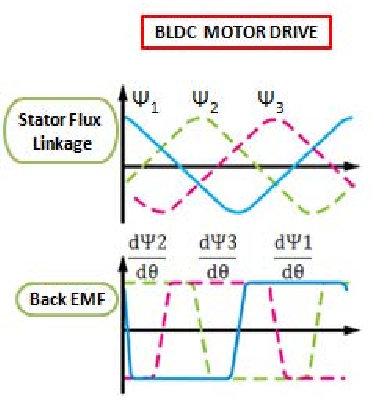
\includegraphics[scale=0.7]{./3_Stand_der_Technik/Abbildungen/BLDC_Back-EMF_1}
			\caption{Back-EMF BLDC-Maschine\cite{Rode2023}}
	\end{figure}
		
	\subsubsection{Permanent erregte Synchronmaschine (PMSM-Maschine)}
		Die PMSM-Maschine isst vom Aufbau fast gleich wie die BLDC-Maschine, nur sind die Magneten im Rotor anders angeordnet. Diese Maschine kann nur mit FOC-Regelung(siehe \ref{Feldorientierte Regelung}) angesteuert werden, welche in der Regel etwas teuer und aufw�ndiger ist. Sie wird mithilfe von einem sinusf�rmigen Drehfeld geregelt und gibt auch ein sinusf�rmiges Back-EMF zur�ck. Sie ist effizienter als die BLDC Maschine und kann auch bei sehr niedrigen und sehr hohen Drehzahlen ohne Probleme verwendet werden. Sie wird verwendet wenn es n�tig ist Drehzahl oder Drehmoment genau zu kontrollieren.\cite{Rode2023}
		
	\begin{figure}[H]
			\centering
			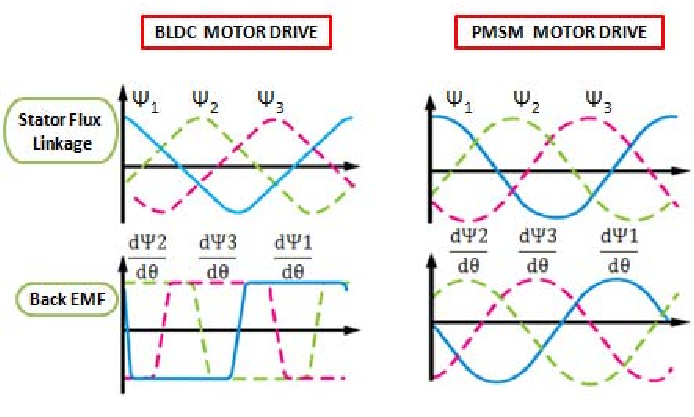
\includegraphics[scale=0.5]{./3_Stand_der_Technik/Abbildungen/PMSM_Back-EMF_1}
			\caption{Back-EMF PMSM-Maschine\cite{Rode2023}}
	\end{figure}
		
	\subsubsection{Fremderregte Synchronmaschine (FSM-Maschine)}
		Die fremderregte Synchronmaschine hat nun im Rotor statt Permanentmagneten Erregerwicklungen, welche entweder durch Schleifringe oder �ber einen Luftspalt induziert Energie �bertragen bekommen. Sie werden gro�teils im Generatorbetrieb eingesetzt, da die erzeugte Leistung einfach geregelt werden kann und sie �ber ihren gesamten Leistungsbereich sehr effizient sind.
	
	\subsubsection{Reluktanzmaschine}
		Bei der Reluktanzmaschine besteht der Rotor der Maschine aus Elektroblech. Es wird nicht wie bei �blichen Maschinen das Prinzip der Lorentzkraft sondern ausschlie�lich das der Reluktanzkraft angewandt. Aufgrund dessen hat dieser Motor eine eher geringe Leistungsdichte, ist aber im Gegenzug sehr g�nstig zu fertigen und zu k�hlen.\cite{oswos.com2024}
	